\documentclass[UTF8,11pt,a4paper,fontset=windows]{ctexart}
\usepackage[margin=2.25cm]{geometry}
\usepackage{amsmath,amssymb,bm,booktabs,tabularx,array,graphicx}
\usepackage{caption,enumitem,float,placeins}
\usepackage[hidelinks]{hyperref}
\usepackage{fancyhdr}
\graphicspath{{assets/}}
\captionsetup{font=small,labelfont=bf}
\setlength{\parindent}{2em}
\setlength{\parskip}{0.18em}
\linespread{1.16}
\setlength{\emergencystretch}{2em}
\numberwithin{equation}{section}
\pagestyle{fancy}
\fancyhf{}
\fancyhead[L]{\small 大语言模型人类偏好数据的长度与格式关联分析}
\fancyhead[R]{\small 修订稿 v2}
\fancyfoot[C]{\thepage}
\setlength{\headheight}{15pt}
\newcolumntype{Y}{>{\raggedright\arraybackslash}X}
\newcommand{\OR}{\mathrm{OR}}
\title{\heiti 大语言模型人类偏好数据的长度与格式关联分析\\[0.3em]
\large ——基于配对 Logistic 模型的审计应用}
\author{程豪\quad 梁斯祯\quad 李嘉帅\quad 姜弼达\quad 翁祖成\quad 姚博晟\\
\small 中央民族大学理学院，北京 100081}
\date{}
\begin{document}
\maketitle
\thispagestyle{plain}
\begin{center}\small
基金项目：国家自然科学基金青年科学基金项目（72001197）；\\
中央民族大学创新训练项目青苗计划（QMRP2025110352）
\end{center}

\noindent\textbf{摘要：}针对大语言模型评价中回答形式与人类选择相互交织的问题，构建基于配对比较的偏好数据审计流程。以 LMArena 公开数据的 108,154 个唯一会话首轮评价为基础，对其中 78,959 对明确胜负记录，采用配对检验及含模型身份对比项的 Logistic 回归，联合分析长度对数比与标题、列表、粗体密度差，并通过英语和单轮子集检查敏感性。结果表明：不等长配对中较长回答获胜比例为 62.37\%；控制可观测任务信息及模型身份后，长度指标每标准差的优势比为 1.6196，粗体密度呈较稳定的正关联，标题关联较弱且对子集敏感，列表密度未获得明确关联证据。另以观测变量广义路径模型保留 SEM 探索：经粗体的关联乘积在三个子集中方向一致，标题通路对样本敏感，列表通路区间跨零。进一步按长度比构建审计分层，长度接近与长度比超过 2 的配对中，较长回答获胜比例分别为 52.46\% 和 69.06\%。据此提出包含明确胜负与未决评价的分层复核方案，为偏好数据质量管理提供量化依据。上述结果属于观察性关联，应用示例不构成标签错误识别或去偏成效验证。

\noindent\textbf{关键词：}大语言模型；人类偏好；配对比较；Logistic 回归；探索性路径分析；数据审计

\begin{center}
\large\bfseries Length and Formatting Associations in Human Preference Data for Large Language Models\\[0.3em]
\normalsize An Audit Application Using a Paired Logistic Model
\end{center}
\noindent\textbf{Abstract:} This study develops a paired-comparison workflow for auditing the association between response form and human choice in large language model evaluation. The analysis uses 108,154 first-evaluation records from unique sessions in a public LMArena dataset, including 78,959 pairs with a decisive outcome. Paired tests and logistic regression with model-identity contrasts jointly examine the log token ratio and differences in heading, list, and bold-formatting densities. English-language and single-turn subsets provide sensitivity checks. Among unequal-length decisive pairs, the longer response wins in 62.37\% of cases. After adjustment for observed task information and model identity, the odds ratio per standard deviation of the length measure is 1.6196. Bold density shows a relatively stable positive association, whereas the heading association is weaker and subset-sensitive; list density has no clear statistical support. An exploratory observed-variable generalized path model further describes candidate associations: the product through bold density remains positive across subsets, the heading pathway is subset-sensitive, and the list-path intervals include zero. These products do not identify causal mediation. A descriptive audit illustration groups pairs by their length ratio. The longer-response win proportions are 52.46\% for near-equal-length pairs and 69.06\% for pairs with a length ratio above two. The resulting strata support a review plan covering both decisive and non-decisive evaluations. These findings are observational associations, and the audit illustration does not establish label errors or validate debiasing effectiveness.

\noindent\textbf{Key words:} large language models; human preference; paired comparison; logistic regression; exploratory path analysis; data audit

\section{引言}
大语言模型评价常采用成对比较：对同一用户问题展示两个候选回答，由用户选择较优者。该方式能够直接记录实际使用中的相对偏好，Chatbot Arena 等平台据此开展众包评价与模型比较\cite{chiang}。然而，一个回答被选中并不等于其所有可观察特征都具有同样的质量含义。较长回答可能提供更多必要信息，也可能包含重复解释；标题、列表和粗体可能改善信息组织，也可能仅改变文本外观。对评价数据使用者而言，需要判断选择结果与这些形式特征之间存在多大关联，从而决定哪些配对应进入进一步复核。

已有研究从不同角度讨论偏好信号的构成。Li 等\cite{li}通过细粒度属性分析比较人类与大语言模型的偏好，表明总体选择背后包含多种评价维度。Dubois 等\cite{dubois}利用回归控制长度因素，改进自动评价指标对长度差异的处理。Zhang 等\cite{zhang}进一步考察列表、粗体等格式模式，说明格式与偏好学习之间的关系值得独立研究。这些工作为偏好数据审计提供了依据，但人类评价与自动评价器输出是不同的研究对象，对自动评价器的校正效果不能直接转化为人类选择中的因果结论。

在真实成对数据中，长度与格式分析还面临两个相互联系的问题。其一，格式计数随文本扩展而变化，仅比较胜者与败者的格式总量，难以判断关联来自格式本身还是文本规模。其二，不同模型的输出习惯、任务分布和被选择概率可能同时不同，忽略模型身份会使形式指标吸收模型间差异。因此，实际分析既要保持成对比较单位的一致性，也要在同一回归中联合纳入长度、格式和可观测背景信息。

本文以 LMArena 公开人类偏好数据为对象，研究三个问题：明确胜负配对的长度与格式差异如何分布；联合调整可观测变量后，哪些关联仍有统计支持；这些结果如何转化为可操作的审计分层。方法上，将长度对数比、格式密度差与模型身份对比项放入同一 Logistic 模型，并结合配对检验和敏感性分析评估结果。同时保留 SEM 框架下的观测变量探索性路径分析，描述长度、格式与选择的候选关联结构。应用上，使用真实样本构建长度分层报告，给出固定复核预算下的抽样方案。本文的贡献在于将配对建模与评价数据复核衔接起来，并明确不同格式指标的证据差异。研究目标限定为观察性关联及其审计用途，形式编辑的因果效果需由独立干预设计检验。

\section{数据与指标构造}
\subsection{数据来源与样本边界}
研究使用 \texttt{lmarena-ai/arena-human-preference-140k} 的本地冻结数据\cite{dataset}，共 7 个原始分片、135,634 条记录。数据同时包含会话标识、评价次序、双方对话、胜负标签及长度和格式元数据。本文按会话首轮评价建立比较单位，检查角色交替、两侧用户输入轨迹一致性、文本有效性、标签完整性及计数合法性。通过筛选后，对仍存在多条候选记录的会话整体排除，得到每个唯一会话一条记录的分析集。

按首次失败原因互斥计数，排除非首轮评价 27,319 条、语言异常 30 条、空或无效文本内容 109 条、会话记录歧义 22 条，最终保留 108,154 条。评价结果包括 A 胜 39,042 条、B 胜 39,917 条、平局 16,574 条、双方差 12,621 条。后两类保留用于描述和审计分层，不并入二元胜负模型；因此，回归样本为 78,959 对明确胜负记录。其分析目标是该筛选总体中的相对选择，而不是所有平台交互中的偏好。

首轮评价与单轮对话需要区分：首轮评价记录内部仍可能包含多轮用户与模型交互，长度和格式由该评价记录的汇总字段表示。限制为首轮有助于减少评价历史与当前测量混杂，但不保证全部计量误差被消除。不同会话仍可能来自同一用户或相同提示词，故会话唯一性不能直接作为观测相互独立的证据。

\subsection{结果变量与形式指标}
对第 $i$ 个明确胜负配对，令 $Y_i=1$ 表示 A 侧胜出，$Y_i=0$ 表示 B 侧胜出。记双方回答 token 总量为 $L_{Ai}$、$L_{Bi}$，二者均为正数。长度指标定义为
\begin{equation}
 x_{Li}=\log\frac{L_{Ai}}{L_{Bi}}.
\end{equation}
与绝对差相比，对数比描述相对长度差异，并在交换双方后改变符号。例如，200 对 100 tokens 与 2,000 对 1,000 tokens 对应相同的长度比。该度量不把相同的绝对差视为相同的相对扩展，也不能替代任务所需信息量的测量。

记格式类型 $f\in\{H,B,S\}$ 分别代表标题、粗体和列表，双方格式计数为 $C_{fAi}$、$C_{fBi}$。定义每千 token 密度差
\begin{equation}
 x_{fi}=1000\left(\frac{C_{fAi}}{L_{Ai}}-\frac{C_{fBi}}{L_{Bi}}\right).
\end{equation}
格式计数沿用上游元数据：标题为 h1--h6 计数之和，列表为有序与无序列表计数之和，粗体为两种标记计数之和。本文未重新实现 Markdown 解析器，故这些指标表示上游识别规则下的形式数量，不等于经人工验证的结构质量或视觉效果。密度可以减少文本规模对格式总量的直接影响，但仍共享长度分母，不能据此认为长度与格式已完全分离。

描述检验使用胜者减败者的差值；回归始终保持原始 A/B 方向，不按照胜负重新排列解释变量。主模型将四个形式指标在相应分析子集中分别标准化，即 $z_{ki}=(x_{ki}-\bar x_k)/s_k$，其中 $s_k$ 采用分母为该子集样本数的标准差。

\begin{table}[htbp]\centering\small
\caption{主要变量及统计含义}\label{tab:vars}
\begin{tabularx}{\textwidth}{p{2.8cm}Y Y}
\toprule
变量 & 定义与来源 & 解释边界\\
\midrule
胜负 $Y_i$ & A 胜为 1，B 胜为 0 & 排除平局与双方差后的条件总体\\
长度 $x_{Li}$ & 双方 token 总量的对数比 & 相对文本规模，不代表信息增益\\
格式 $x_{fi}$ & 标题、粗体、列表每千 token 密度差 & 依赖上游计数，共享长度分母\\
任务及提示词 & 任务标签、七类提示词属性、输入长度、轮数及语言 & 不是逐条回答内容质量评分\\
模型身份 & A、B 两侧模型指示变量之差 & 控制模型间平均差异，不等于题目级质量控制\\
\bottomrule
\end{tabularx}
\end{table}

\subsection{控制变量与敏感性子集}
任务信息包括创意写作、指令遵循、数学和代码标签。七类提示词属性对应复杂性、创造性、领域知识、问题求解、现实情境、具体性和技术准确性需求，其取值来自任务标注，不能解释为回答已达到相应质量标准。另纳入用户输入 token 数的 $\log(1+L_U)$、对话轮数和语言虚拟变量；各分析子集中频数低于 100 的语言合并为低频类别。

模型身份采用双方模型指示变量的差表示，不使用由本批胜负标签估计的模型胜率作为解释变量。为检查语言混合及对话轮次口径的影响，另对英语样本 42,001 对和单轮对话样本 67,608 对拟合相同类型模型。二者与全量样本重叠，属于敏感性检查；子集间指标标准差不同，不能直接将 OR 差异解释为同一原始单位的关联变化。

\section{配对统计模型与审计方法}
\subsection{配对差异检验}
令 $D_i$ 为某项特征的胜者值减败者值，剔除零差后的配对数为 $n_*$，正差数为 $n_+$。以
\begin{equation}
 \widehat q=\frac{n_+}{n_*}
\end{equation}
描述不等值配对中胜者特征更大的比例。在独立配对及正负差等概率的零假设下，$n_+\sim\mathrm{Binom}(n_*,1/2)$，据此进行双侧符号检验并计算精确二项区间。对格式是否出现的二元指标，只比较双方存在性不一致的配对，形成精确 McNemar 检验。零差数量与总样本量同时报告，避免以不同分母比较特征强弱。

作为补充，以非零差绝对值的平均秩计算配对秩二列相关
\begin{equation}
 r_{\mathrm{rb}}=\frac{W_+-W_-}{W_++W_-},
\end{equation}
其中 $W_+$ 和 $W_-$ 为正差与负差的秩和。该量用于描述差异方向及相对强度。Wilcoxon 符号秩检验也保留在补充结果中；由于差值分布对称性未得到保证，不将其无条件表述为中位数检验，也不依赖它识别因果关系。

\subsection{含模型身份对比项的 Logistic 模型}
设 $p_i=\Pr(Y_i=1\mid\bm z_i,\bm X_i,m_{Ai},m_{Bi})$，构建
\begin{equation}\label{eq:logit}
 \log\frac{p_i}{1-p_i}=\alpha+\beta_Lz_{Li}+\beta_Hz_{Hi}
 +\beta_Bz_{Bi}+\beta_Sz_{Si}+\bm\gamma^\top\bm X_i
 +\theta_{m_{Ai}}-\theta_{m_{Bi}}.
\end{equation}
其中 $\bm X_i$ 为控制变量，$\theta_m$ 为模型身份参数，选定一个参考模型并令其参数为零。模型身份项沿用 Bradley--Terry 配对比较的参数差形式\cite{bradley}，在此基础上加入记录层特征与控制变量。截距及记录层控制项允许 A 侧获胜概率随观测背景变化，因此本文模型不是只含模型能力参数的纯排名模型。

令 $\bm v_i$ 为完整设计向量、$\bm\eta$ 为参数向量，通过最大化 Bernoulli 对数似然估计参数：
\begin{equation}
 \ell(\bm\eta)=\sum_{i=1}^{n}\left[Y_i\bm v_i^\top\bm\eta
 -\log\{1+\exp(\bm v_i^\top\bm\eta)\}\right].
\end{equation}
实现中先检查设计矩阵满秩，再检验迭代收敛和参数有限性。全量、英语和单轮模型均通过上述检查；对应设计矩阵秩分别为 90、69 和 89。这些检查保证数值结果满足当前估计程序要求，不等于模型设定已经充分捕捉全部选择因素。

采用 HC0 夹心协方差估计标准误。若 $\widehat W=\mathrm{diag}\{\widehat p_i(1-\widehat p_i)\}$，则
\begin{equation}
 \widehat{\mathrm{Var}}(\widehat{\bm\eta})=
 (V^\top\widehat WV)^{-1}
 \left[\sum_{i=1}^{n}\bm v_i\bm v_i^\top(Y_i-\widehat p_i)^2\right]
 (V^\top\widehat WV)^{-1}.
\end{equation}
这里仍以观测间独立为工作假设。HC0 不处理同一用户跨会话或重复提示词带来的聚类依赖，相应区间应在该限制下解释。

\subsection{关联量解释与多重比较}
标准化指标 $z_k$ 的条件优势比为 $\OR_k=\exp(\beta_k)$，表示在模型中其他变量保持不变时，该指标增加一个标准差对应的获胜优势之比。OR 不等于概率倍数，也不意味着实际添加某种格式后必然产生同样变化。若需概率尺度的辅助描述，平均局部导数为
\begin{equation}
 \overline{\partial p/\partial z_k}=\frac{\widehat\beta_k}{n}
 \sum_{i=1}^{n}\widehat p_i(1-\widehat p_i).
\end{equation}
其含义是拟合概率的平均局部斜率，不是实际增加一个标准差的离散概率变化。

多重比较采用 Holm 方法\cite{holm}。配对分析中，全量、英语、单轮及 16 种任务标签组合的全部符号与 McNemar 检验共同构成一个家族；补充 Wilcoxon 检验未参与该校正。回归中，三个模型的 12 个焦点系数共同构成另一个家族。按升序排列原始 $p$ 值后，调整值为
\begin{equation}
 \widetilde p_{(j)}=\min\left\{1,\max_{1\leq k\leq j}(M-k+1)p_{(k)}\right\}.
\end{equation}
本文采用双侧 0.05 水平，表图中的 95\% 区间为逐项区间，不是同时置信区间。对于浮点下溢产生的零值，以 $p<0.001$ 呈现，不将其解释为概率严格等于零。任务组合的小样本结果仅保留供追溯，不据此开展细碎的实质推断。

\subsection{审计分层规则}
模型分析用于识别需要关注的特征，具体抽样则使用可直接计算且不依赖胜负方向的指标。定义无方向长度比
\begin{equation}\label{eq:ratio}
 R_i=\frac{\max(L_{Ai},L_{Bi})}{\min(L_{Ai},L_{Bi})}\geq1,
\end{equation}
以 $R_i\leq1.25$、$1.25<R_i\leq2$ 和 $R_i>2$ 构成三层。阈值用于展示接近、中等和较大长度差异，是本次分析阶段确定的解释性规则，不是预注册阈值或已验证的最优风险界限。规则不将原始标签判为正确或错误，也不因结果显著而自动调整样本权重。

审计报告同时输出各层总量、明确胜负数、平局与双方差数量，以及不等长明确胜负配对中的较长回答获胜比例。这样既可观察形式差异，也可检查二元建模排除的评价是否集中在特定层中。第6节基于真实记录给出应用示例。

\section{实证结果与敏感性分析}
\subsection{未调整的配对差异}
在 78,959 对明确胜负记录中，187 对等长，78,772 对不等长；较长回答获胜 49,130 对，比例为 62.37\%，95\% 精确二项区间为 [62.03\%, 62.71\%]。胜者减败者的中位长度差为 125 tokens，配对秩二列相关为 0.3278。前一比例只使用不等长配对，中位数则使用全部明确胜负配对，二者回答的问题不同。

\begin{table}[htbp]\centering\small
\caption{全量样本的配对差异摘要}\label{tab:paired}
\begin{tabular}{lrrrr}
\toprule
特征与口径 & 非零差配对数 & 正差比例（\%） & $r_{\mathrm{rb}}$ & Holm $p$\\
\midrule
长度计数 & 78,772 & 62.37 & 0.3278 & $<0.001$\\
标题计数 & 47,046 & 58.79 & 0.2080 & $<0.001$\\
标题密度 & 49,087 & 55.30 & 0.1164 & $<0.001$\\
粗体计数 & 68,357 & 60.26 & 0.2608 & $<0.001$\\
粗体密度 & 70,187 & 55.80 & 0.1547 & $<0.001$\\
列表计数 & 66,959 & 59.13 & 0.2334 & $<0.001$\\
列表密度 & 69,296 & 50.33 & 0.0046 & 1.0000\\
\bottomrule
\end{tabular}
\par\smallskip\footnotesize 注：正差为胜者特征大于败者；各行分母仅为相应特征的非零差配对。全部明确胜负配对数为 78,959，零差数可由总数减去第二列得到。
\end{table}

表\ref{tab:paired}表明，计数与密度不能混为同一证据。胜者列表计数较多的比例为 59.13\%，但列表密度较高的比例仅为 50.33\%，校正后未获显著支持。标题和粗体在密度口径下仍呈正向差异，但秩二列相关较计数口径减小。这说明格式比较对文本规模的处理敏感；它不证明列表仅由长度生成，也不能将显著的格式密度差直接等同于不合理偏好。

\subsection{联合回归中的调整关联}
表\ref{tab:reg}报告全量样本四个焦点系数。长度对数比每增加一个标准差，其调整后 OR 为 1.6196，95\% 区间为 [1.5804, 1.6597]。全量长度指标标准差约为 1.0224，故这个单位不是增加一个 token，也不是长度恰好翻倍。相同模型条件下，长度对数比增加 1.0224，对应原长度比乘以约 2.780；该换算仅说明回归尺度。

\begin{table}[htbp]\centering\small
\caption{全量联合 Logistic 模型的焦点关联}\label{tab:reg}
\begin{tabular}{lrrrr}
\toprule
变量 & $\widehat\beta$ & OR & 95\% 逐项区间 & Holm $p$\\
\midrule
长度对数比 & 0.4822 & 1.6196 & [1.5804, 1.6597] & $<0.001$\\
标题密度差 & 0.0278 & 1.0282 & [1.0092, 1.0476] & 0.0212\\
粗体密度差 & 0.0541 & 1.0556 & [1.0339, 1.0778] & $<0.001$\\
列表密度差 & $-0.0129$ & 0.9872 & [0.9703, 1.0043] & 0.5631\\
\bottomrule
\end{tabular}
\par\smallskip\footnotesize 注：样本数为 78,959；四项指标联合入模并分别标准化。模型调整任务、提示词属性、输入长度、轮数、语言及模型身份，标准误为 HC0。
\end{table}

粗体密度的 OR 为 1.0556，标题密度为 1.0282，均在全量模型中呈正关联；列表密度区间跨越 1。即使标题和粗体通过多重比较校正，其在各自标准化尺度上的关联量仍小于长度项，不能只凭大样本下的显著性把格式描述为主导选择的因素。对于全量样本，标题、粗体及列表密度差的标准差分别约为 5.2319、18.3675 和 18.3726 次/千 tokens，这也说明标准化 OR 不能直接转换为“添加一次格式”的收益。

联合纳入可观测变量后长度关联仍然存在，表明它不完全被本模型的控制项吸收。然而，模型身份只控制不同模型的平均差异，不能测量同一模型在具体题目上的回答质量。准确性、覆盖率和冗余程度未被独立标注，因而长度仍可能同时代表信息充分性及其他未观测因素。这里的“调整”是给定模型设定后的条件比较，而非剥离内容质量后的纯长度效应。

\subsection{英语与单轮子集}
图\ref{fig:reg}展示三个分析样本的估计。英语和单轮子集的长度 OR 分别为 1.5847 和 1.6436，校正后均有统计支持；粗体密度 OR 分别为 1.0815 和 1.0581，同样保持正关联。因此，在本次可检查的语言和轮次口径下，长度与粗体的方向较稳定。

\begin{figure}[htbp]\centering
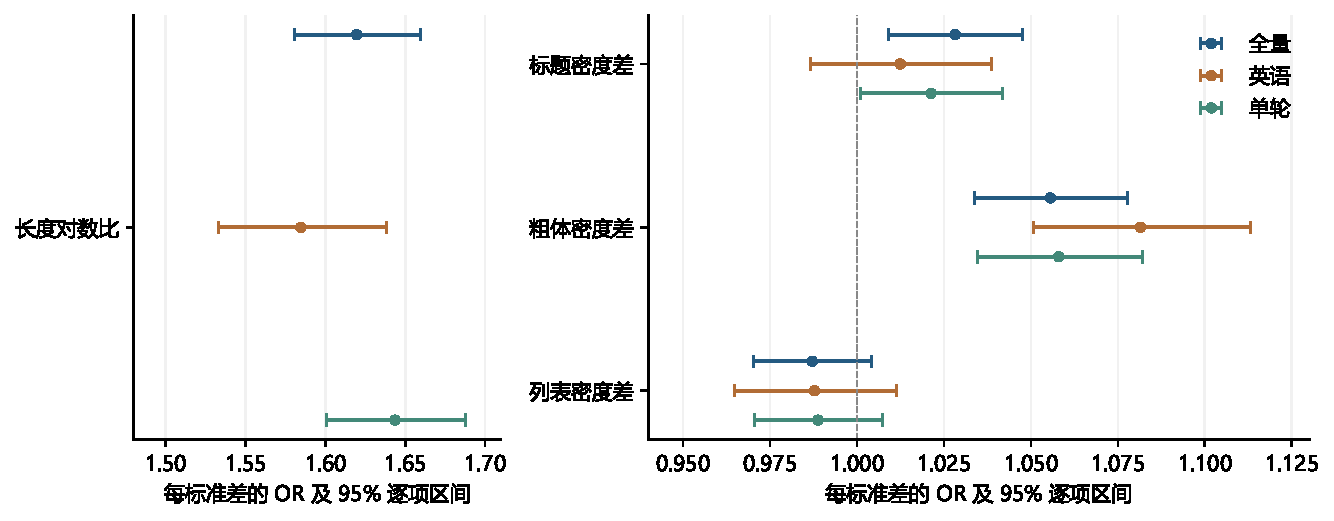
\includegraphics[width=\textwidth]{adjusted_associations.pdf}
\caption{全量、英语与单轮样本的调整关联。左右面板横轴范围不同；区间为逐项 95\% 区间，各子集分别标准化。}\label{fig:reg}
\end{figure}

标题密度在英语子集中的 OR 为 1.0124，95\% 区间为 [0.9868, 1.0388]；单轮子集 OR 为 1.0213，逐项区间为 [1.0011, 1.0420]，但 Holm 校正后的 $p=0.1954$。因此，标题不宜与粗体合并为“稳定格式效应”。列表密度在两个子集中均缺少明确关联证据。逐项区间排除 1 与校正后不显著并不矛盾，因为二者采用不同的多重比较口径。

这些子集分析没有消除选择偏差或提供独立外部验证。尤其是子集分别标准化，且样本大量重叠，点估计差异只能作为敏感性描述。对于重复提示词、用户相关性、极端长度以及非线性关系，当前模型仍需进一步检验；不能把三次同向估计理解为全部稳健性问题均已解决。

\FloatBarrier
\section{探索性路径分析}
\subsection{观测变量 SEM 框架与估计}
为保留结构方程模型（SEM）的探索性尝试，本文进一步考察长度、格式与选择之间的候选关联通路。采用无潜变量的广义路径框架：三个连续格式方程由最小二乘估计，二元选择方程由 Bernoulli--Logistic 模型估计。该框架属于分方程的观测变量路径分析，没有潜变量测量模型，不沿用将二元结果作为连续正态变量处理的旧 SEM。路径方向为事后提出的工作设定，并非由数据识别出的时间或因果顺序。

对 $k\in\{H,S,B\}$，设
\begin{equation}
 z_{ki}=\alpha_k+a_kz_{Li}+\bm\gamma_k^\top\bm X_i
 +\theta_{k,m_{Ai}}-\theta_{k,m_{Bi}}+\varepsilon_{ki}.
\end{equation}
结果方程沿用式\eqref{eq:logit}，将其中长度系数记为 $c$，格式系数记为 $b_k$。三个格式方程使用相同的长度和控制变量，允许其残差相关，不设置格式间的有向路径。样本、A/B 方向、标准化与控制项均与主分析一致；没有从同一批胜负标签构造所谓模型能力代理，也没有按显著性删除列表路径。结果方程与主分析相同，因而不能将其再次拟合视为独立验证。

构造跨方程的 HC0 夹心协方差，保留同一配对在各方程中估计得分的相关性。七条关注路径在三个子集中形成 21 项 Holm 校正家族。对 $q_k=a_kb_k$，从系数的联合渐近正态分布进行 50,000 次参数模拟，报告乘积的 2.5\% 和 97.5\% 分位数；随机种子为 20260921。模拟区间条件于样本标准化尺度，为逐项区间，未作多重比较校正，也不是记录重采样 Bootstrap 区间。

乘积 $q_k$ 仅描述给定方程设定下的候选关联通路，不是概率变化或自然间接效应。由于结果方程采用非线性 logit 链接，不将 $c+\sum_kq_k$ 解释为约简模型的总效应，不计算中介比例。本次分方程估计未构建共同协方差结构的拟合检验，故不报告 CFI、TLI 或 RMSEA，也不借用旧 SEM 的拟合指标。

\subsection{探索结果及解释边界}
在全量 78,959 对样本中，长度指向标题、列表、粗体密度的标准化斜率分别为 0.1541、0.1357、0.1391。指向选择的标题、列表、粗体系数分别为 0.0278、$-0.0129$、0.0541，长度系数为 0.4822，均位于 log-odds 尺度；这些量不能与格式方程斜率直接比较大小。

\begin{table}[htbp]\centering\small
\caption{探索性路径乘积及 95\% 逐项模拟区间}\label{tab:paths}
\begin{tabular}{llrr}
\toprule
样本 & 候选通路 & 乘积 & 区间\\
\midrule
全量 & 长度$\to$标题$\to$选择 & 0.00429 & [0.00142, 0.00716]\\
全量 & 长度$\to$列表$\to$选择 & $-0.00175$ & [$-0.00412$, 0.00056]\\
全量 & 长度$\to$粗体$\to$选择 & 0.00753 & [0.00462, 0.01045]\\
英语 & 长度$\to$标题$\to$选择 & 0.00198 & [$-0.00213$, 0.00609]\\
英语 & 长度$\to$列表$\to$选择 & $-0.00157$ & [$-0.00460$, 0.00142]\\
英语 & 长度$\to$粗体$\to$选择 & 0.01000 & [0.00632, 0.01388]\\
单轮 & 长度$\to$标题$\to$选择 & 0.00317 & [0.00014, 0.00620]\\
单轮 & 长度$\to$列表$\to$选择 & $-0.00159$ & [$-0.00425$, 0.00104]\\
单轮 & 长度$\to$粗体$\to$选择 & 0.00780 & [0.00472, 0.01095]\\
\bottomrule
\end{tabular}
\par\smallskip\footnotesize 注：全量、英语及单轮样本量分别为 78,959、42,001、67,608。各子集分别标准化且相互重叠；区间未经多重校正。箭头表示探索性模型设定，不能证明因果方向。
\end{table}

表\ref{tab:paths}显示，经粗体的乘积在三组样本中均为正，标题通路在英语样本中的区间跨零，列表通路在三组样本中的区间均跨零。单轮标题乘积的逐项区间虽排除零，其指向选择的路径仍未通过 Holm 校正（$p=0.1954$）；两类判断的统计量和校正口径不同，不能据此宣称标题存在稳定机制。

该探索提示粗体相关通路值得后续独立研究，但不能说明格式传递了长度的因果作用。长度与格式同期测量，格式密度又含长度分母，独立内容质量缺失以及用户和提示词相关性均可能影响结果。当前未检验反向路径、替代测量、非线性及聚类稳健性。探索结果用于提出后续可检验的问题，不替代前述条件关联结果或独立干预验证。

\FloatBarrier
\section{偏好数据审计应用}
\subsection{面向复核的分层报告}
设偏好数据进入后续评价或训练流程前，管理者只能复核有限数量的记录。仅按总体比例随机抽样能够描述总体，却可能使特定形式差异层中的记录较少。本文依据式\eqref{eq:ratio}形成三个长度层，并同时保留明确胜负和平局、双方差。表\ref{tab:audit}为本次冻结数据的实际统计，图\ref{fig:audit}展示各层的较长回答获胜比例。

\begin{table}[htbp]\centering\small
\caption{按无方向长度比构建的审计分层}\label{tab:audit}
\begin{tabular}{lrrrr}
\toprule
长度层 & 保留记录 & 明确胜负 & 未决比例（\%） & 较长者获胜（\%）\\
\midrule
$R\leq1.25$ & 23,536 & 15,964 & 32.17 & 52.46\\
$1.25<R\leq2$ & 37,992 & 27,017 & 28.89 & 59.26\\
$R>2$ & 46,626 & 35,978 & 22.84 & 69.06\\
\bottomrule
\end{tabular}
\par\smallskip\footnotesize 注：未决包括平局与双方差，分母为本层全部保留记录；较长者获胜比例的分母为本层不等长且明确胜负配对，依次为 15,777、27,017 和 35,978。
\end{table}

在长度接近层，较长回答获胜比例为 52.46\%，区间为 [51.67\%, 53.24\%]；中等差异层为 59.26\%，区间为 [58.67\%, 59.84\%]；较大差异层为 69.06\%，区间为 [68.58\%, 69.53\%]。这是一组未调整的分层描述，不是控制其他条件后使回答变长的效果。不同层的内容充分性、任务需求或模型组合可以不同，不能因比例上升便把较大差异层判为偏差样本。

\begin{figure}[htbp]\centering
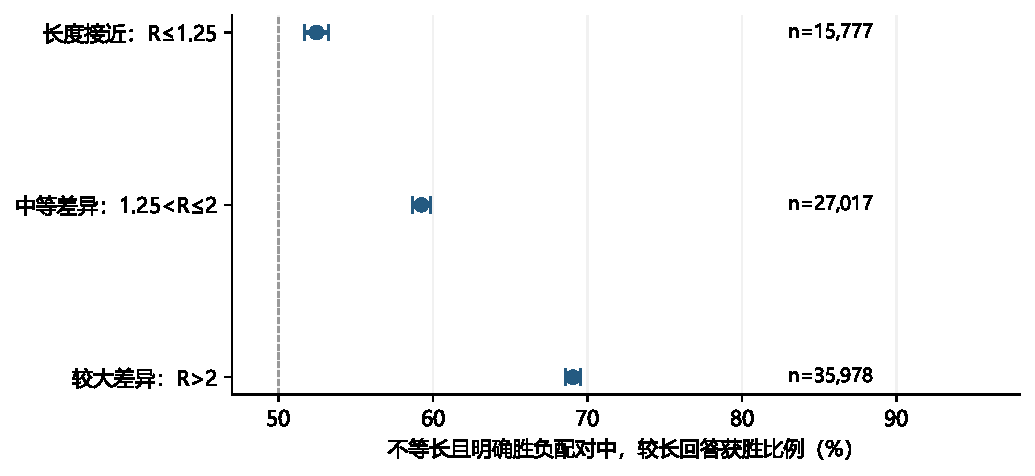
\includegraphics[width=.92\textwidth]{audit_strata.pdf}
\caption{各长度层中较长回答获胜的比例与 95\% 精确二项区间。区间以配对独立为工作假设，未进行多重比较校正。}\label{fig:audit}
\end{figure}

长度分层也揭示了二元分析的样本边界。长度接近层中平局及双方差占 32.17\%，在较大差异层中占 22.84\%；前者比后者高约 9.33 个百分点。若审计只沿用回归中的明确胜负样本，将无法检查这些未决评价是否包含可识别的质量问题。因而实际复核应将未决状态纳入抽样框，不能把排除记录理解为没有分析价值。

作为格式交叉描述，在粗体密度不相等且明确胜负的配对中，粗体密度较高者在三个长度层的获胜比例依次为 49.79\%、51.36\% 和 61.49\%，分母分别为 13,525、23,817 和 32,845。该结果提示总体格式关联可能随长度层的样本构成变化，支持同时检查长度与格式。它没有进一步控制层内残余长度差、任务和模型身份，不应与表\ref{tab:reg}的联合回归量相互替代。

\subsection{固定预算下的复核方案}
上述分层可以转化为具体的抽样任务。例如，在 300 条记录的复核预算下，先向三个长度层各分配 100 条，并在层内按明确胜负、平局、双方差的构成进行随机抽样；若某类样本需单独研究，可事先设定最低抽样数并记录实际纳入概率。等额分配是便于比较各层的方案示例，本文未实际实施人工复核，也未验证其优于比例分配或随机抽样。

复核者需同时评价双方内容的正确性、相关性、信息覆盖及组织清晰度，尽可能隐藏原始胜负标签，并记录复核选择与理由。不能把复核者不同意原选择直接当成标签错误：偏好本身可能存在合理差异，应另设独立可核验的内容标准。由于标题或列表可能承载任务所需结构，自动删去格式再比较也未必保持语义和任务条件不变。

若用分层样本估计该审计总体的争议比例，应恢复原抽样权重。记层 $h$ 的总体数量为 $N_h$、复核样本量为 $b_h$、争议指标为 $a_{hj}\in\{0,1\}$，在层内简单随机抽样条件下可使用
\begin{equation}
 \widehat A=\sum_{h=1}^{H}\frac{N_h}{N}
 \left(\frac{1}{b_h}\sum_{j=1}^{b_h}a_{hj}\right).
\end{equation}
若进一步按评价状态分层，则 $h$ 应表示长度层与状态的交叉层；若采用不等概率抽样，则需使用相应纳入概率加权。直接平均三个长度层的争议比例，会把当前样本中人数不同的层赋予相同权重，改变所估计的总体。

\subsection{应用价值与验证范围}
本例已经完成从配对数据到分层统计的可复现转换：使用不依赖 A/B 位置的长度比，输出各层记录量、未决构成及形式与选择的描述关联，并提供可实施的复核分配规则。这使“关注长度与格式”成为有明确抽样框和结果口径的操作，而不仅是原则性建议。

应用上，长度和粗体可作为持续监测的候选特征；标题需要结合具体场景复核，列表密度不宜单独作为剔除条件。关联强弱不能替代标签可靠性判断，也不能由当前 OR 直接推导去偏权重。尤其不能为了使较长回答获胜比例接近 50\% 而删样，因为真实内容优势也可能产生这一关联。

本文没有开展复核效率、奖励模型训练或榜单校准实验，因此应用结论限于审计流程与数据示例。要评价分层方案的实际收益，需要在独立样本和相同复核预算下比较不同抽样方案，报告争议发现率、复核一致性及其不确定性，并避免同一用户或重复提示词跨验证组。只有获得此类证据后，才能讨论审计效率是否改善。

\section{结论与局限}
本文保留 SEM 框架下的探索性路径分析：经粗体的关联乘积在三个重叠样本中方向一致，标题通路具有样本敏感性，列表通路区间跨零。该分析仅描述候选关联结构，不支持因果中介或机制识别结论。

本文针对大语言模型成对评价数据，联合分析长度对数比及标题、粗体、列表密度差。在明确胜负且不等长的样本中，较长回答获胜比例为 62.37\%；调整可观测任务信息及模型身份后，长度与粗体呈较稳定的正关联，标题关联较弱且对子集敏感，列表密度未获得明确关联证据。结果表明，评价数据中的形式关联需要分指标、分口径报告，不能以格式计数差异代替独立格式作用的判断。

基于真实记录构建的长度分层，将统计结果衔接到抽样复核流程：各层较长回答获胜比例及未决评价构成均有差异，支持同时保留明确胜负、平局和双方差开展审计。该应用提供了可计算的分层规则和总体恢复公式，尚不构成审计效率或偏好训练质量改善的证明。

研究局限包括单一平台及冻结样本的外部有效性、缺乏独立回答质量测量、上游长度与格式测量误差、重复用户与提示词的相关性、时间变化及平局排除带来的选择问题。当前线性 logit 设定和密度分母耦合也可能影响解释。后续应优先补充内容复核、聚类依赖与非线性敏感性检验，并在独立数据上评价审计流程。本文结论应理解为有条件的观察性关联，而非长度或排版干预的因果效应。

\FloatBarrier
\begin{thebibliography}{99}\small
\bibitem{chiang} CHIANG W L, ZHENG L, SHENG Y, et al. Chatbot Arena: An Open Platform for Evaluating LLMs by Human Preference[EB/OL]. (2024-03-07)[2026-09-21]. \url{https://arxiv.org/abs/2403.04132}.
\bibitem{li} LI J, ZHOU F, SUN S, et al. Dissecting Human and LLM Preferences[C]//Proceedings of the 62nd Annual Meeting of the Association for Computational Linguistics (Volume 1: Long Papers). 2024: 1790--1811. \url{https://doi.org/10.18653/v1/2024.acl-long.99}.
\bibitem{dubois} DUBOIS Y, GALAMBOSI B, LIANG P, et al. Length-Controlled AlpacaEval: A Simple Way to Debias Automatic Evaluators[EB/OL]. (2024-04-06)[2026-09-21]. \url{https://arxiv.org/abs/2404.04475}.
\bibitem{zhang} ZHANG X, XIONG W, CHEN L, et al. From Lists to Emojis: How Format Bias Affects Model Alignment[C]//Proceedings of the 63rd Annual Meeting of the Association for Computational Linguistics (Volume 1: Long Papers). 2025: 26940--26961. \url{https://doi.org/10.18653/v1/2025.acl-long.1308}.
\bibitem{dataset} LMARENA AI. arena-human-preference-140k[DS/OL]. [2026-09-21]. \url{https://huggingface.co/datasets/lmarena-ai/arena-human-preference-140k}.
\bibitem{bradley} BRADLEY R A, TERRY M E. Rank Analysis of Incomplete Block Designs: I. The Method of Paired Comparisons[J]. Biometrika, 1952, 39(3/4): 324--345. \url{https://doi.org/10.1093/biomet/39.3-4.324}.
\bibitem{holm} HOLM S. A Simple Sequentially Rejective Multiple Test Procedure[J]. Scandinavian Journal of Statistics, 1979, 6(2): 65--70. \url{https://www.jstor.org/stable/4615733}.
\end{thebibliography}
\end{document}
